\subsection{GitHubの使い方}
解析ソースコードの共有および測定データの共有にGitHubを使うことを推奨します.必要な情報のほとんどウェブ検索によって得られる(\href{https://tech-blog.rakus.co.jp/entry/20200529/git}{例})と思いますが, 簡単な解説を以下に示します.

\subsubsection{git, GitHubとは}
gitはコマンドライン上でテキストファイル群のバージョン(変更履歴)管理を行うためのツールです.
gitはバージョン管理を図\ref{fig:git_desc}のように行っており, 各開発者の持つローカルリポジトリと共有のためのリモートリポジトリが存在します\cite{github}.リポジトリとはバージョン管理の対象となるファイル群のことを指します.開発者はリモートリポジトリから最新のソースコードを受け取り, ローカルリポジトリにコピーします.ローカルリポジトリで開発を進め, 変更箇所をリモートリポジトリに渡します.このようにして複数人での開発が可能になります.ここで, リモートリポジトリをホストするサービスとしてGitHubがあります(GitHub以外にもあります).
\begin{figure}
    \centering
    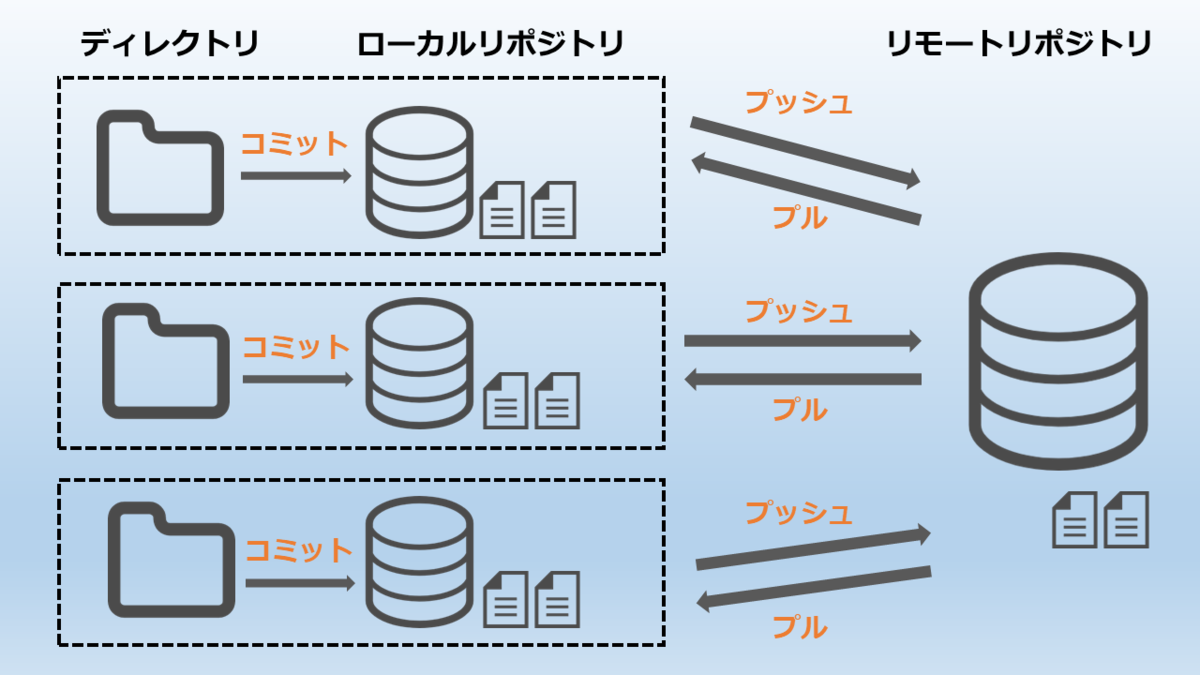
\includegraphics[height=4cm]{git_desc.png}
    \caption{gitの概念図\cite{github}}
    \label{fig:git_desc}
\end{figure}

\subsubsection{gitの簡単な使い方}
\begin{itemize}
    \item リモートリポジトリをローカルマシンにダウンロードする
    \begin{lstlisting}
$ git clone (address)
    \end{lstlisting}
    \item ローカルにあるブランチの一覧を見る
    \begin{lstlisting}
$ git branch
    \end{lstlisting}
    \item ブランチを作る
    \begin{lstlisting}
$ git branch new_branch
    \end{lstlisting}
    \item 別のブランチに移る
    \begin{lstlisting}
$ git chackout new_branch
    \end{lstlisting}
    \item ローカルリポジトリの変更状況を表示する
    \begin{lstlisting}
$ git status
    \end{lstlisting}
    \item 変更をアップする
    \begin{lstlisting}
$ git add modified_file01
$ git add modified_file02
$ git commit -m "commit message"
$ git push origin new_branch
    \end{lstlisting}
    \item メインブランチの変更を現在のブランチに落としてくる
    \begin{lstlisting}
$ git pull origin main
    \end{lstlisting}
\end{itemize}